%!TEX root = ../../main.tex


\begin{figure}[!htb]
\centering
%\hrulefill \\
%\vspace{5pt}
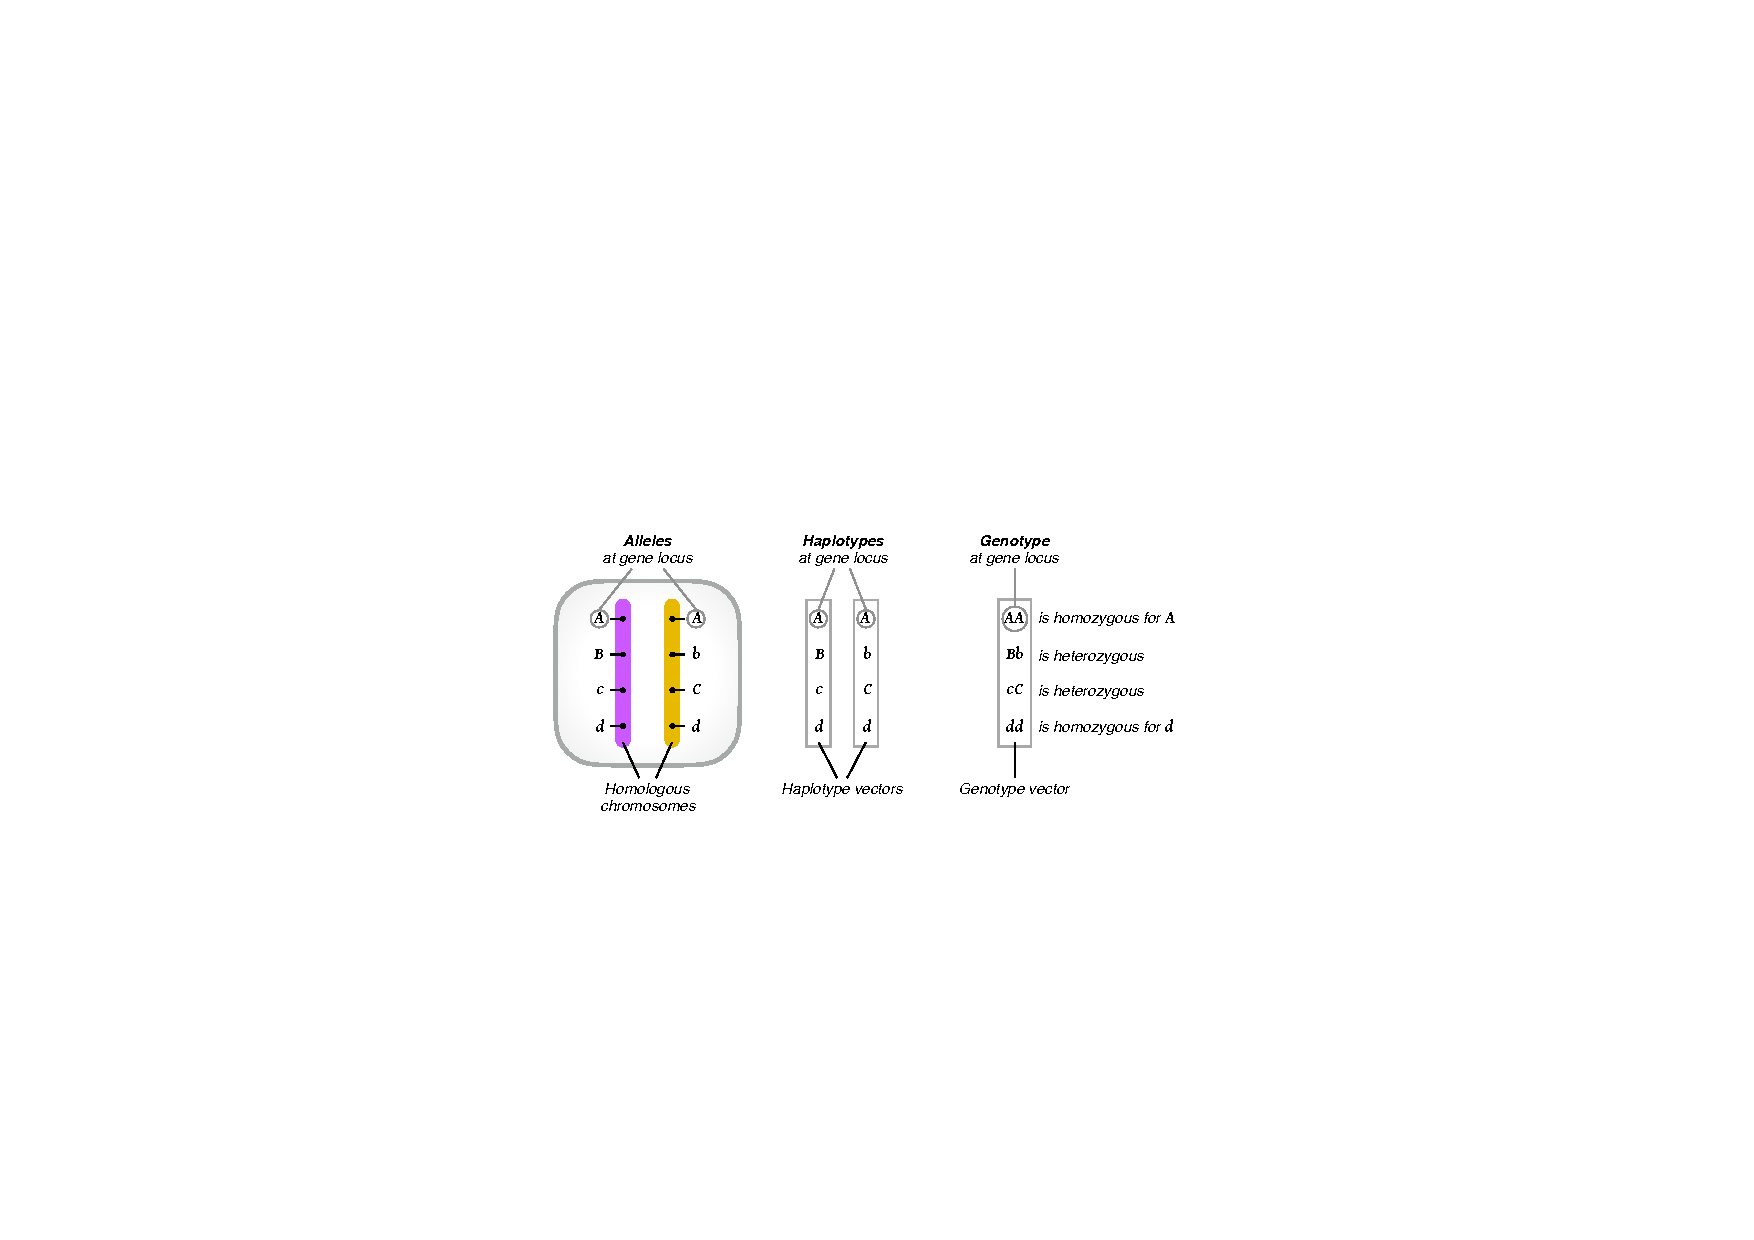
\includegraphics[width=0.8\textwidth]{./img/ch1/info_types}
\Caption{Alleles, haplotypes, and genotypes}
{A pair of homologous chromosomes is shown (\emph{left}) on which \n{4} gene loci are highlighted; labelled as $A$, $B$, $C$, and $D$.
Maternal and paternal chromosomes are shown in \emph{purple} and \emph{yellow} (arbitrarily coloured).
Each gene may have \n{2} allelic states (in this example), distinguished by capitalisation of the label.
Each chromosome has a corresponding haplotype at each locus (\emph{middle}).
Genotypes do not distinguish chromosomes and are represented as the sum of allelic information inherited from both parents (\emph{right}).
Note that the term \emph{haplotype} may refer to the allelic state observed at a single nucleotide or a set of alleles observed along a chromosome.
Likewise, the term \emph{genotype} may refer to the allelic dosage at a single site or a vector of observed genotypic information.}
{fig:info_types}
% \vspace{-5pt}
% \hrulefill%
\end{figure}
